\section{Convolutions} %Jonathan / b-j8508, b-j8510, b-j8512, b-j8515 / Jul 13, 15-17,
In this section, we will talk about the convolutions, and we will focus more about implementation of it in PyTorch. To see the documentation of the \emph{Conv2d} operator in PyTorch, there are a bunch of parameters, like number of channels, kernel size. We want to talk about what exactly those things mean here.
\begin{figure}[H]
\centering
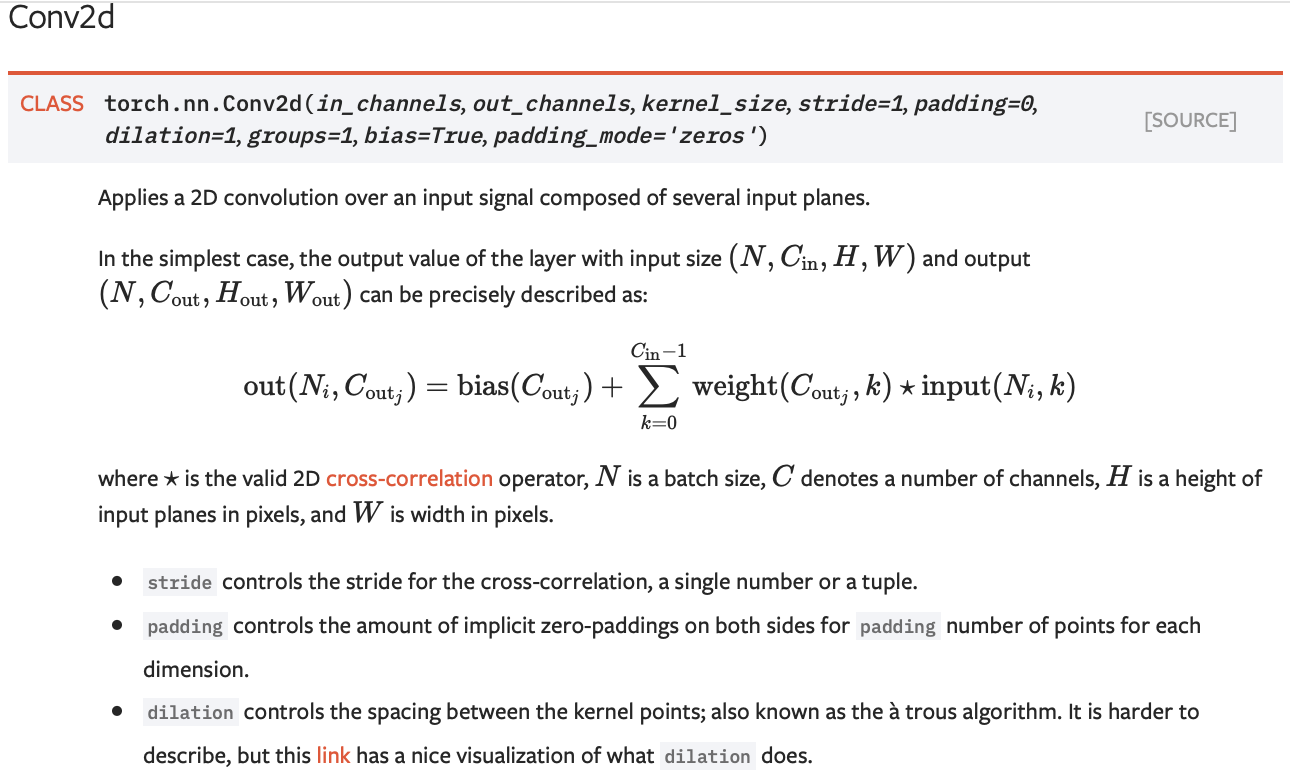
\includegraphics[scale=0.5]{./figures/497Proj_conv2d}
%\caption{}
\end{figure}

So let's first talk about the simplest case with 1 input channel and 1 output channel, which means 1 input and 1 output images. 
\begin{itemize}
\item kernel size
\item stride
\item padding
\item dilation
\end{itemize}

\begin{figure} %\label{mugrid-bi}
\begin{center}
\setlength{\unitlength}{0.445mm}
\begin{picture}(45,45)(50,0)
\linethickness{0.1mm}
\multiput(0,0)(5,0){9}{\line(0,1){40}}
\multiput(0,0)(0,5){9}{\line(1,0){40}}

\multiput(80,15)(5,0){4}{\line(0,1){15}}
\multiput(80,15)(0,5){4}{\line(1,0){15}}

\end{picture}
\setlength{\unitlength}{0.5mm}
\end{center}
\hskip1.1in {Input image $I$} \hskip0.5in {kernel $K$}
%\caption{multilevel grids for piecewise bilinear functions}
\end{figure}

Suppose, we have an n-by-n input image(i.e an n-by-n array of numbers), each of this box represents a real number, and a kernel, which is a much smaller array of numbers, usually 3-by 3 or 5-by-5. 
And the convolution $K * I$ will be a new image, called output image $O$.  Now let's just immediately not worry about what size of this image is. We just talk about how to fill in its entries. Now we want to form this convolution w.r.t. the kernel $K$ with the image $I$, what will be the top lefthand entry? How to determine it? Since we have a 3-by-3 kernel, we take the dot product of kernel $K$ and the first 3-by-3 top left block of the image, and it gives the first top left entry value of the output image. 

\begin{figure} %\label{mugrid-bi}
\begin{center}
\setlength{\unitlength}{0.445mm}
\begin{picture}(45,45)(50,0)
\linethickness{0.1mm}
\multiput(-20,40)(5,0){1}{\line(0,-1){30}}
\multiput(-20,40)(0,5){1}{\line(1,0){30}}
\multiput(-15,35)(5,0){1}{\line(0,1){5}}
\multiput(-15,35)(0,5){1}{\line(-1,0){5}}

\put(30,20){$\gets$}

\multiput(47,42)(5,0){4}{\line(0,-1){15}}
\multiput(47,27)(0,5){4}{\line(1,0){15}}

\multiput(65,40)(5,0){6}{\line(0,-1){25}}
\multiput(65,15)(0,5){6}{\line(1,0){25}}

\multiput(50,0)(5,0){9}{\line(0,1){25}}
\multiput(50,0)(0,5){6}{\line(1,0){40}}

%\multiput(50,0)(5,0){9}{\line(0,1){40}}
%\multiput(50,0)(0,5){9}{\line(1,0){40}}

\multiput(120,25)(5,0){4}{\line(0,1){15}}
\multiput(120,25)(0,5){4}{\line(1,0){15}}

\end{picture}
\setlength{\unitlength}{0.5mm}
\end{center}
\hskip 1in {Output $O$} \hskip0.55in {Input $I$} \hskip0.55in {Kernel $K$}
%\caption{multilevel grids for piecewise bilinear functions}
\end{figure}

Similarly of the next entry in the right, we just shift the 3-by-3 block of $I$ over by 1 to the right, and take the dot product of the kernel with it.

\begin{figure} %\label{mugrid-bi}
\begin{center}
\setlength{\unitlength}{0.445mm}
\begin{picture}(45,45)(50,0)
\linethickness{0.1mm}
\multiput(-20,40)(5,0){1}{\line(0,-1){30}}
\multiput(-20,40)(0,5){1}{\line(1,0){30}}
\multiput(-15,35)(5,0){2}{\line(0,1){5}}
\multiput(-10,35)(0,5){2}{\line(-1,0){5}}
 
\put(30,20){$\gets$}
 
\multiput(50,40)(5,0){2}{\line(0,-1){15}}
\multiput(50,25)(0,5){4}{\line(1,0){5}}

\multiput(55,42)(5,0){4}{\line(0,-1){15}}
\multiput(55,27)(0,5){4}{\line(1,0){15}}

\multiput(70,40)(5,0){5}{\line(0,-1){15}}
\multiput(70,25)(0,5){4}{\line(1,0){20}}

\multiput(50,0)(5,0){9}{\line(0,1){25}}
\multiput(50,0)(0,5){6}{\line(1,0){40}}

%\multiput(50,0)(5,0){9}{\line(0,1){40}}
%\multiput(50,0)(0,5){9}{\line(1,0){40}}


\multiput(120,25)(5,0){4}{\line(0,1){15}}
\multiput(120,25)(0,5){4}{\line(1,0){15}}

\end{picture}
\setlength{\unitlength}{0.5mm}
\end{center}
\hskip 1in {Output $O$} \hskip0.55in {Input $I$} \hskip0.55in {Kernel $K$}
%\caption{multilevel grids for piecewise bilinear functions}
\end{figure}

And the rest of output entries are similarly. Based on this, take the convolution of an n-by-n input image  with a  3-by-3 kernel, and we can get the output image with dimension $(n-2) \times (n-2)$. And in this simplest case, the kernel size is $3\times 3$ and stride and dilation are $1$. And there is no padding. So what do these parameters mean?
\begin{itemize}
\item kernel size is the dimension of the kernel matrix, and it doesn't have to be square.
\item stride tells us if we move one pixel in the output image, how far do I shift the kernel in the input image to get the dot product. (In our example, we shift 1 at a time.). And the large stride will give a small output. 
\item padding tells you how many zeros to add around the input images.
\item dilation tells you, to take the dot product, when we move 1 in the kernel, how much do I move in the block of input image.
\end{itemize}
Notice that both of stride and padding, we can have different values in each directions.
And there is a nice digit illustration of convolution \url{https://github.com/vdumoulin/conv_arithmetic}.
One more thing have to mention is the convolutions also have a bias term. The bias term is just added to $K*I$.
Now, what happens with more than one input/output channels.
Suppose we have $n$ input channels and $m$ output channels. Then 
\begin{itemize}
\item there will be $n\times n$ kernels, denoted by $K_{ij}$, for $i =1,\ldots,n$ and $j=1,\ldots,m$. 
\item input is $n$ images, denoted by $I_1^{\rm in}, \ldots, I_m^{\rm in}$
\item $m$ output images, denoted by $I_1^{\rm out}, \ldots, I_m^{\rm out}$
\end{itemize}
Here, 
$$I_{i}^{\rm out} = \sum_{j=1}^n K_{ij}*I_j^{\rm in}$$
Basically, densely connected across channels. Every channel talks to every channels via some kernels. And also, we have different bias term for every output channels.
So this is how convolutional layers work, now let's look what happens when you construct the \emph{Conv2d} class and what the weights look like. Suppose that we construct a convolution layer with 1 input channel, 1 output channel, kernel size with 3, and all the other augments are default, like the simplest example.  
\begin{python}
import torch
import torch.nn as nn
layer = nn.Conv2d(1,1,3)
parameters = list(layer.parameters())
\end{python}
%What the parameters of this class look like? 
We can call \emph{parameters = list(layer.parameters())} to see that the parameters of the convolution layer we just constructed are a $3\times 3$ kernel and a bias term. And in the simplest case, take $n=10$, which means the input image is $10\times 10$. We can check the dimension of the output channel is $(n-2)\times (n-2)$.
\begin{python}
x = torch.randn(1,1,10,10)
layer(x).size()
\end{python}
It will return \emph{[1,1,8,8]}. 
To add more channels, 
\begin{python}
layer = nn.Conv2d(2,2,3) # 2 input channels, 2 output channels and 3-by-3 kernel
parameters = list(layer.parameters())
\end{python}
Now, we can see the parameters for the new convolution layer contains 4 kernels with size $3\times 3$ and 2 bias term.

%MNIST Experiment: use a sequence of convolutional layers followed by a linear layer to classify MNIST. 


\section{Max pooling} 
In this section, we will introduce max pooling. We already learned the multigrid methods and the relationship between convolution neural network and multigrid methods. When implementing multigrid methods, we have a sequence of coarse and fine grids. In CNN, you want images to get the grids from one to another, and people use max pooling.
Input: An image I with multiple channels \\
Output: a smaller, ``lower-resolution" image with the same number of channels
\begin{itemize}
\item Channels do not interact, pooling is done on each channel independently.
\end{itemize}
The parameters, kernel size, stride, padding and dilation, in max pooling play the same roles as in convolution.
\begin{itemize}
\item Notice that basically there will be no kernel here, because all this important is the size.
\end{itemize}

\begin{figure}[H]
\centering
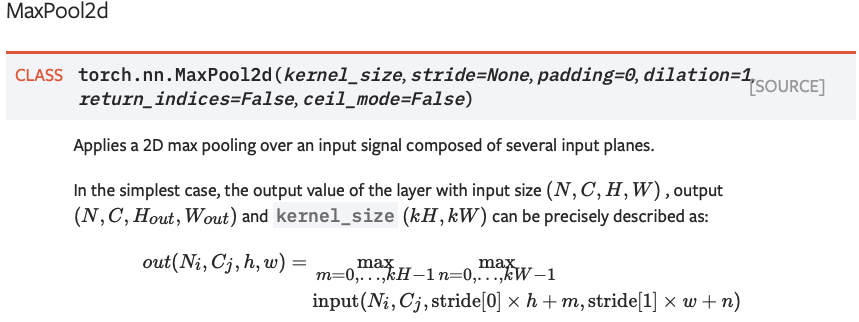
\includegraphics[scale=0.75]{./figures/497Proj_maxpooling}
\end{figure}

Like the convolution operator, the max pooling with kernel size 2 works as
\begin{figure} %\label{mugrid-bi}
\begin{center}
\setlength{\unitlength}{0.445mm}
\begin{picture}(45,45)(50,0)
\linethickness{0.1mm}
\multiput(-10,40)(5,0){1}{\line(0,-1){30}}
\multiput(-10,40)(0,5){1}{\line(1,0){30}}
\multiput(-5,35)(5,0){1}{\line(0,1){5}}
\multiput(-5,35)(0,5){1}{\line(-1,0){5}}

\put(30,20){$\stackrel{\textrm{take the maximum of the block}}{\longleftarrow}$}

\multiput(97,42)(5,0){3}{\line(0,-1){10}}
\multiput(97,32)(0,5){3}{\line(1,0){10}}

\multiput(110,40)(5,0){7}{\line(0,-1){40}}
\multiput(110,0)(0,5){9}{\line(1,0){30}}

\multiput(100,0)(5,0){9}{\line(0,1){30}}
\multiput(100,0)(0,5){7}{\line(1,0){40}}


\end{picture}
\setlength{\unitlength}{0.5mm}
\end{center}
\hskip 1in {Output $O$} \hskip0.55in {Input $I$} \hskip0.55in {Kernel $K$}
%\caption{multilevel grids for piecewise bilinear functions}
\end{figure}
Max pooling has the same parameters with the convolution. Basically, it is the same thing, instead of taking some convolution with the kernel, you just take the maximal value of these entries to get the corresponding entry of output. In particular, there is no model parameters associated with the max pooling layers.

And let's just talk about stride again. The PyTorch default for max pooling is to set the stride equal to the kernel size. So the default behavior is, if you kernel size is 2, to reduce the dimension in each direction by 2. It is similar to taking it to a coarse grid.

And let's start with creating a 6-by-6 torch tensor.
\begin{python}
import torch
import torch.nn as nn
x = torch.randn(1,1,6,6)
\end{python}
The first two augments of $x$ represent the batch size and the number of channels.
So, let just create a max pooling layer. 
\begin{python}
max_pool = nn.MaxPool2d(2)
\end{python}
Now, if the max pooling is applied to x, then what is the dimension of \emph{max\_pool(x)}?
The answer is $3\times 3$ since the stride is default. And let's set the stride to be something different, say stride=1, what now?
\begin{python}
max_pool = nn.MaxPool2d(2, stride=1)
\end{python}
Call \emph{max\_pool(x)} and see the difference. Now, the size of output will be $5\times 5$. Because, we just shift the window over by 1 each time.

Actually, max pooling is a non-linear function, you can just construct a neural network consisting entirely convolution and max pooling, you don't need ReLU. And also a piecewise linear function, behaves similar to the ReLU. There is an example of max pooling convolution network.
\begin{python}
# maxconv.py
import torch 
import torchvision
import torchvision.transforms as transforms
import torch.nn as nn
import torch.nn.functional as F
import torch.optim as optim


class MaxConvNet(nn.Module):
    def __init__(self):
        super(Net, self).__init__()
        self.conv_step = nn.Sequential(
        nn.Conv2d(1, 4, 2),
        nn.MaxPool2d(kernel_size=(2, 2), stride=(1,1)),
        nn.Conv2d(4, 8, 4),
        nn.MaxPool2d(kernel_size=(4, 4), stride=(1,1)),
        nn.Conv2d(8, 15, 4),
        nn.MaxPool2d(kernel_size=(4, 4)))
        self.dense_linear = nn.Linear(4 * 4 * 15, 10)

    def forward(self, x):
        x = self.conv_step(x)
        x = x.view(-1, 4 * 4 * 15)
        x = self.dense_linear(x)
        return x
\end{python}
Notice that there are no ReLU, but the max pooling introduce the non-linearity. That allows it to fit the data. We can create an instance of the network. 
\begin{python}
import torch
from maxconv import MaxConvNet
model = MaxConvNet()
\end{python}
And you can check that even it's a small network, it still has less than 5 thousand parameters. 
\begin{python}
sum(p.numel() for p in model.parameters())
\end{python}
And also can test its accuracy. You can try different activation function to see what will happen.


\section{Dropout} 
This is an idea invented by Hinton, 2012. 
It is an integral component of AlexNet.
And it can be thought of as a regularization which improve the generalization accuracy.

What is the idea? Consider the neural network model $f(x, \theta) = NN(x, \theta)$, where $\theta$ are the parameters in each layer. We try to learn a function $f$ that is of the neural network form by optimizing a loss function $$\min_\theta\ L(f(x,\theta)).$$

Idea behind dropout is to consider a whole family of network. 
Given a network, we randomly remove some neurons and all of the corresponding connections.

for each neuron, remove with probability $p$.
produces a random new neural network
let $f(x,\theta) = \textrm{average of } \tilde{NN}(x,\theta)$ over all sampled network $\tilde{NN}$, in mathematical $\mathbb{E}_\sigma(\tilde{NN}(x,\theta))$. 
However we can not really calculate the expectation over the exponential large number of neural networks. 
To make this tractable, two approximations: 
\begin{enumerate}
\item $\min_\theta\ L(\mathbb{E}_\sigma (NN_\sigma (x, \theta))) \approx \mathbb{E}_\sigma L(NN_\sigma (x,\theta))$ \\
Now we can use SGD by randomly sampling
$\sigma$ (i.e. a collection of neurons to remove)
and performing SGD on the result smaller network. Don't update weights that were removed. (gradients at removed weights are 0) \\
\item When testing, replace $\mathbb{E}_\sigma(NN_\sigma(x,\theta))$ by moving the expectation into the weight. For each neuron, at the training time, multiply the output of the neuron by $p$.
\end{enumerate}

In PyTorch, we can find there are two functions 
\emph{model.train()} and \emph{model.eval()} to set the neural network in training or evaluation modes. Now we see one reason is sometimes we need different operations in these two different process.

So I recommend adding dropout in you network, seeing what happens. The idea is because you average all of the different neural networks. What if these neurons die, and you network still works well. Looking at the average of a bunch of pruned networks, makes this process more robust to the generalization accuracy. And in practice, dropout works very well.

Now, let's see how to implement the dropout and batch normalization.
In PyTorch, we can create this dropout layers.
\begin{figure}
\centering
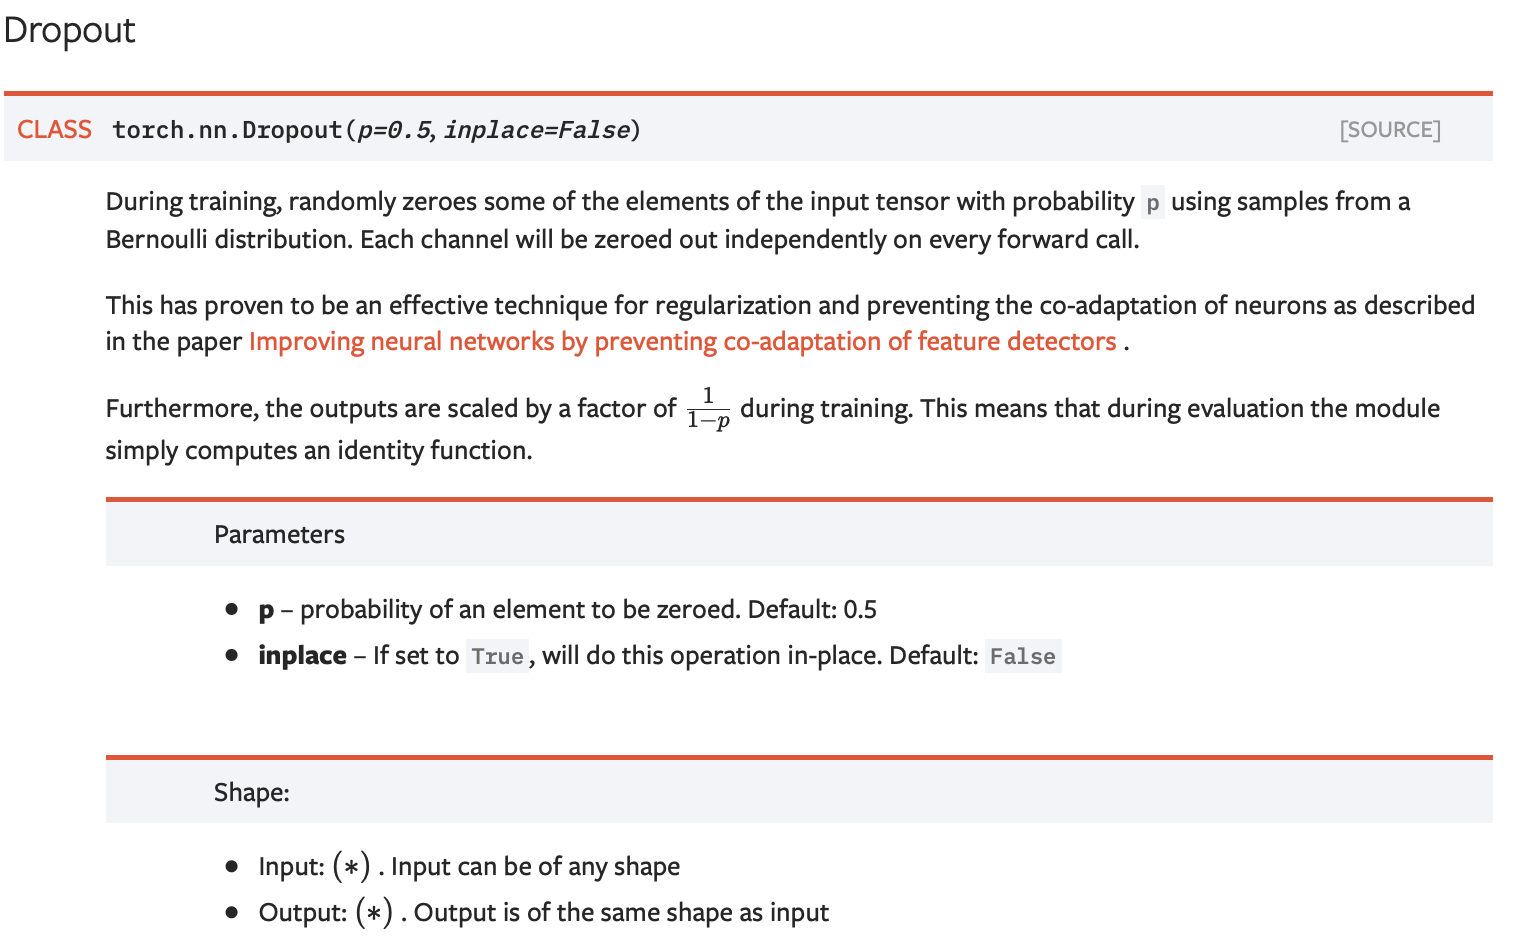
\includegraphics[scale=0.4]{./figures/497Proj_dropout}
\end{figure}
Here we can see, how to construct it, really all you need to pass it is a single probability. That is the probability that the neurons in that layers is dropped out. For example, notice that the values that go into each neuron is the output of previous layer. If you apply a dropout, you just take the value $x$ and pass it through the dropout layer before fill it in the next layer. 
%It will drops out some of the inputs, essentially removes some of these neurons with probability $p$. 
The essential thing dropout does is take the input and set its entry to zero with probability $p$.

So all dropout does is when it see its input, it randomly set it to zero with probability $p$, and rescale everything that wasn't set to zero by $\frac{1}{1-p}$ in the training.
And then during evaluation/testing, it doesn't do anything. 

Now let's see how to add the dropout in our CIFAR example. We only need to modify the \emph{Net} class part as follows:
\begin{python}
class Net(nn.Module):
    def __init__(self):
        super(Net, self).__init__()
        self.conv1 = nn.Conv2d(3, 6, 5)
        self.pool = nn.MaxPool2d(2, 2)
        self.conv2 = nn.Conv2d(6, 16, 5)
        self.fc1 = nn.Linear(16 * 5 * 5, 120)
        self.fc2 = nn.Linear(120, 84)
        self.fc3 = nn.Linear(84, 10)
        self.dropout = nn.Dropout(p=0.3)

    def forward(self, x):
        x = self.pool(F.relu(self.conv1(x)))
        x = self.pool(F.relu(self.conv2(x)))
        x = x.view(-1, 16 * 5 * 5)
        x = self.dropout(F.relu(self.fc1(x)))
        x = F.relu(self.fc2(x))
        x = self.fc3(x)
        return x
\end{python}
We create a dropout layers in \emph{\_\_int\_\_} and put it between the first and the second linear layers. Now in this network, before the second linear layer, dropout is applied. It's the same thing as removing  randomly a bunch of neurons in the second layer. You can add this dropout layer anywhere else as well.

And when start training, you should be sure you model is set to the training mode, and in evaluation mode before testing. So
\begin{python}
conv_net = Net()

criterion = nn.CrossEntropyLoss()
optimizer = optim.SGD(net.parameters(), lr=0.001, momentum=0.9)

net.train()

for epoch in range(2):  # loop over the dataset multiple times

    running_loss = 0.0
    for i, data in enumerate(trainloader, 0):
        # get the inputs; data is a list of [inputs, labels]
        inputs, labels = data

        # zero the parameter gradients
        optimizer.zero_grad()

...

net.eval()

correct = 0
total = 0
with torch.no_grad():
    for data in testloader:
        images, labels = data
        outputs = net(images)
        _, predicted = torch.max(outputs.data, 1)
        total += labels.size(0)
        correct += (predicted == labels).sum().item()

\end{python}
So, we need to add \emph{net.train()} before training and \emph{net.eval()} before testing. When we call \emph{net.train()}, this cause all these dropout layers to get activate, and when we call \emph{net.eval()} it turns off that dropout layers. And it the same for the batch normalization and other things that perform different in training and testing.


\section{Batch Normalization}
Similar to the dropout, Batch Normalization (BN) is also a ``regularization" technique which improves generalization accuracy. Then idea of BN is to make 
the neuron outputs to be distributed ``nicely".
To achieve this, we shift and rescale the outputs at each neuron (during the training process) with the mean and standard deviation.

Given some $x_1, \ldots, x_k\in\mathbb{R}$ shift and rescale the $x$, so that mean = 0, standard deviation std = 1. 
\begin{itemize}
\item subtract $\mu = \frac{1}{n}\sum_{i=1}^n x_i$ from each point
\item divide by $\sigma = \sqrt{\frac{1}{n-1}\sum_{i=1}^n (x_i-\mu)^2}$
\end{itemize}
And do this across each mini-batch.
 
Normalize the outputs of each neuron for all data points in a mini batch so these values have mean=0 and std=1.
However, mean=0, std=1 might not be right (the real/best distribution might not be mean=1, std=1), so we introduce two new parameters for each neuron, one for shifting and one for rescaling, which control the actual mean, std of its output.
There are two steps in the training process. 
\begin{itemize}
\item Shift and rescale with the sample mean and std, 
\item and shift and rescale again with the new tunable parameters.
\end{itemize}

How do we evaluate the network after training? (Now we don't have mini-batches, the network will have one image as input at a time, so there are no mean and std. So we don't now how to do the first step.) In the evaluating/testing process,
\begin{itemize}
\item fix $\mu$, $\sigma$ to a weighted average of the values seen for each mini-batch during training, and shift and rescale with these two fixed values in the first step.
\end{itemize}

Notice that, as with dropout, the forward step(evaluating the model/network) is different during training and testing.
So be sure to switch between training and eval mode!

\subsection{Implementation for batch normalization} 
Let's see the batch normalization. There are three different type of batch normalization in PyTorch, for 1d, 2d and 3d data. If you have vectors, you would like to use \emph{BatchNorm1d}
\begin{figure}[H]
\centering
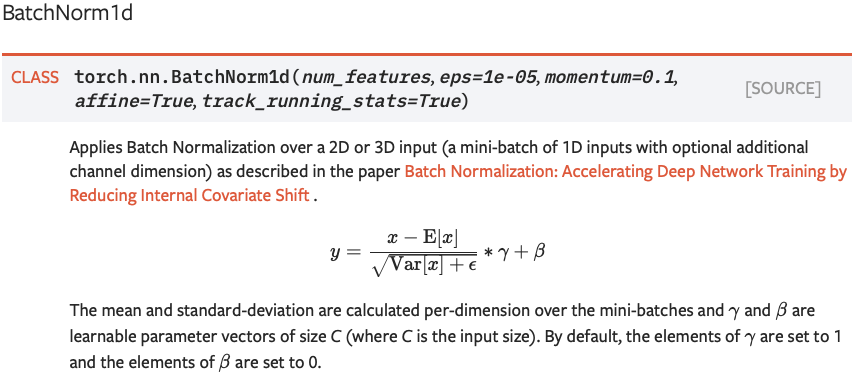
\includegraphics[scale=0.7]{./figures/497Proj_bn1d}
\end{figure}
and use \emph{BatchNorm2d} for image/matrix. 
\begin{figure}[H]
\centering

\includegraphics[scale=0.7]{./figures/497Proj_bn2d}
\end{figure}
And you will want to add it after your layers that will cause to normalize it and train. And you should, the same, think about to switch the training/evaluating mode. For example,
\begin{python}
class Net(nn.Module):
    def __init__(self):
        super(Net, self).__init__()
        self.conv1 = nn.Conv2d(3, 6, 5)
        self.pool = nn.MaxPool2d(2, 2)
        self.conv2 = nn.Conv2d(6, 16, 5)
        self.fc1 = nn.Linear(16 * 5 * 5, 120)
        self.fc2 = nn.Linear(120, 84)
        self.fc3 = nn.Linear(84, 10)
        self.dropout = nn.Dropout(p=0.3)
        self.bn_image = nn.BatchNorm2d(6)
        self.bn = nn.BatchNorm1d(84)

    def forward(self, x):
        x = self.bn_image(self.pool(F.relu(self.conv1(x))))
        x = self.pool(F.relu(self.conv2(x)))
        x = x.view(-1, 16 * 5 * 5)
        x = self.dropout(F.relu(self.fc1(x)))
        x = self.bn(F.relu(self.fc2(x)))
        x = self.fc3(x)
        return x
\end{python}
And the parameters here. The number of features, what is explained in the documentation, is equal to the number of channels for \emph{BatchNorm2d}, which should be 6 after the first convolution layer. Similar in the fully connected part, we want to take \emph{BatchNorm1d}, and the parameter here is the dimension of the input vector, which is 84 after the second linear layer.

And of course, we need to use \emph{net.train()} to set model to training mode before training process, and call \emph{net.eval()} to set model to evaluating mode before test when batch normalization involved.




